\documentclass{article}
\usepackage[utf8]{inputenc}
\usepackage{amsmath}
\usepackage{amssymb}
\usepackage{tikz}

\begin{document}
\date{}
\maketitle

\begin{center}
    \fbox{Cercle trigo}\\ 
    \vspace{0.3cm}
    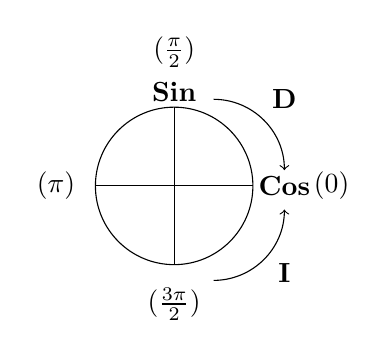
\begin{tikzpicture}
        \draw (0,0) circle (1);
        \draw (0,1.2) node{\textbf{Sin}};
        \draw (0,-1) -- (0,1); % Vertical
        \draw (1.4,0) node{\textbf{Cos}};
        \draw (-1,0) -- (1,0); % Horizontal
        
        \draw (0,1.7) node{($\frac{\pi}{2}$)};
        \draw (-1.5,0) node{($\pi$)};
        \draw (0,-1.5) node{($\frac{3\pi}{2}$)};
        \draw (2,0) node{(0)};
        
        \draw[<-] (1.4, 0.2) arc (0:90:0.90); % Dérive
        \draw (1.4,1.1) node{\textbf{D}};
        \draw[->] (0.5,-1.2) arc (-90:0:0.90); % Intergale
        \draw (1.4,-1.1) node{\textbf{I}};
    \end{tikzpicture}\\
\end{center}

\begin{tabular}{cc}
    \fbox{\textbf{Sinus}}\\
    \begin{tikzpicture} 
        \draw[->] (0,0) -- (0,2);
        \draw[->] (0,0) -- (2,0);
    \end{tikzpicture}&  \\
\end{tabular}


\newpage
\begin{center}
    \textit{Dérivées}\\
    \begin{tabular}{|c|c|c|}
        \hline
        Fonction & Domaine de dérivabilités & Dériviée\\
        \hline
        ln(x) & $\mathbb{R}^{+,*}$	&  $\frac{1}{x}$ \\ 
        \hline
        $e^x$ & $\mathbb{R}$	&  $e^x$ \\ 
        \hline
        $\frac{1}{x}$ & $\mathbb{R}^*$	&  $-\frac{1}{x^2}$ \\ 
        \hline
        $\sqrt{x}$ & $\mathbb{R}^{+,*}$	&  $\frac{1}{2\sqrt{x}}$ \\ 
        \hline
        $\sqrt{x^\alpha}, \alpha \in \mathbb{R}^{+,*}$ & $\mathbb{R}^{+,*}$	&  $ \alpha x^{\alpha - 1} $ \\ 
        \hline
        $ \cos{x} $ & $\mathbb{R}$	&  $ -\sin{x} $ \\ 
        \hline
        $ \tan{x} $ & $ ] -\frac{\pi}{2} + k\pi ; \frac{\pi}{2} +k\pi [, k\in\mathbb{Z} $ & $ 1+\tan{x}^2 = \frac{1}{cos{x}^2} $\\
        \hline
        \arccos{x} & ]-1;1[ & $-\frac{1}{\sqrt{1-x^2}}$ \\
        \hline
        \arcsin{x} & ]-1;1[ & $\frac{1}{\sqrt{1-x^2}}$ \\
        \hline
        \arctan{x} & $\mathbb{R}$ & $\frac{1}{\sqrt{1-x^2}}$ \\
        \hline
    \end{tabular}
\end{center}

\thispagestyle{empty}

\begin{center}
    \begin{tabular}{|c|c|}
    \hline
    Opération & Dériviée\\
    \hline
    f+g & f'+g'\\
    \hline
    f\times g & f'g + fg' \\
    \hline
    $\frac{f}{g}$ & $\frac{f'g - fg'}{g^2}$ \\
    \hline 
    $g \circ g$ & $f'g' \circ f$\\
    \hline
    $\frac{1}{u}$ & $-\frac{u'}{u^2}$ \\
    \hline
    $u^n$ & $nu'u^{n-1}$\\
    \hline
    $\sqrt{u}$ & $\frac{u'}{2\sqrt{u}}$ \\
    \hline
    $e^u$ & $u'e^{u}$\\
    \hline
    $\ln{u}$ & $\frac{u'}{u}$ \\
    \hline
    $ \sin{u} $ & $u'\sin{u}$ \\
    \hline
    \cos{u} & $-u'\sin{u}$\\
    \hline
    \end{tabular}
\end{center}
\newpage
\begin{center}
    \textit{Primitives}\\
    \begin{tabular}{|c|c|c|}
    \hline
    Fonction& Intervalle d'intégration & Primitive \\
    \hline
    $(x-a)^n , n\in \mathbb{N}, a\in \mathbb{R}$ & $ \mathbb{R}$ & $\frac{1}{n+1}(x-a)^{n+1}$ \\
    \hline
    $\frac{1}{x-a}, a\in \mathbb{R}$& $] -\infty;a[ou]a;+\infty [$& $ln(|x-a|)$\\
    \hline
    $ \frac{1}{(x-a)^n}, a \in \mathbb{R} \geqslant 2 $ & $] -\infty;a[ou]a;+\infty [$ & $-\frac{1}{(n-1)(x-a)^{n-1}}$\\
    \hline
    $\cos{ax}, \in \mathbb{R}\baskslash {0}$ & $\mathbb{R}$ & $\frac{1}{a} sin(ax)$ \\
    \hline
    $\sin{ax}, \in \mathbb{R}\baskslash {0}$ & $\mathbb{R}$ & $-\frac{1}{a} cos(ax)$ \\
    \hline
    $\tan{x}$ & $] j\pi -\frac{\pi}{2}, k\pi + \frac{\pi}{2} [, k\in \mathbb{Z}$ & $-ln(|\cos{x}|)$ \\
    \hline
    $ln(x)$ & $\mathbb{R}^{+,*}$ & $ -ln(|\cos{x}|) $ \\
    \hline
    $e^{ax}, a\in \mathbb{R} \baskslash {0}$ & $\mathbb{R}$ & $\frac{1}{a}e^{ax}$ \\
    \hline
    $(x-a)^x, a\in \mathbb{R}, \alpha\in \mathbb{R} {-1}$ & $] a;\infty [$ & $ \frac{1}{\alpha+1}(x-a)^{\alpha+1} $\\
    \hline
    $a^x,a>0$ & $\mathbb{R}$ & $\frac{1}{ln(a)}a^x$ \\
    \hline
    $ \frac{1}{x^2+1} $ & $ \mathbb{R} $ & $ arctan(x)$ \\
    \hline
    $ \sqrt{x-a}, a \in \mathbb{R} $ & $ ] a;+\infty [ $ & $ \frac{2}{3}(x-a)^{\frac{3}{2}} $ \\
    \hline
    $\frac{1}{\sqrt{x-a}}, a \in \mathbb{R}$ & $] a;+\infty [$ & $2\sqrt{x-a}$\\
    \hline
    $\frac{1}{\sqrt{1-x^2}}$ & $] -1;1 [$ & $arcsin(x)$ \\
    \hline
    \end{tabular}
\end{center}


\begin{center}
    \textit{Transformation usuelles}\\
    \begin{tabular}{|c|c|}
    \hline
    $f(t)U(t)$ & F(p) \\
    \hline
    f(t)&1\\
    \hline
    $f(t-\tau)$ & $e^{-\tau p}$\\
    \hline
    $ U(t) $ & $\frac{1}{p}$ \\
    \hline
    $at $ & $\frac{a}{p^2}$ \\
    \hline
    $t^2$ & $ \frac{2}{p^2} $ \\
    \hline
    $ t^n $ & $ \frac{n!}{p^{n+1}} $ \\
    \hline
    $e^{\pm at}$ & $\frac{1}{p\mp a}$ \\
    \hline
    $ 1- e^{-\frac{t}{\tau}} $ & $ \frac{1}{p(1-\tau p)} $ \\
    \hline
    $e^{at}t^{n}$ & $ \frac{n!}{(p-a)^n{n+1}} $\\
    \hline
     $\sin{\omega t}$ & $ \frac{w}{p^2+w^2} $ \\
    \hline
    $\cos{\omega t}$ & $\frac{p}{p^2+w^2}$ \\
    \hline
    $sinh(\omega t)$ & $ \frac{w}{p^2+w^2}$ \\
    \hline
    $\cosh{\omega t}$ & $\frac{p}{p^2+w^2}$ \\
    \hline
     $ e^{-at}sin(\omega t) $ & $ \frac{\omega}{(p+a)^2+\omega^2} $ \\
    \hline
     $ e^{-at}cos(\omega t) $ & $ \frac{p+a}{(p+a)^2+\omega^2} $ \\
    \hline
    $\sin{\omega t + \phi}$ & $\frac{psin(\phi) + \omega cos(\phi)}{p^2+w^2}$ \\
    \hline
    \end{tabular}
\end{center}
\thispagestyle{empty}


\end{document}
